\documentclass[aspectratio=169,10pt]{beamer}
\usetheme{default}
\usecolortheme{seahorse}
\setbeamertemplate{navigation symbols}{}
\setbeamertemplate{footline}[frame number]
\usepackage{graphicx, booktabs}
\graphicspath{{../figures/}}
\title{Run\_55 Resist-HV Scan: MM Tracking vs Time-Since-Flash\\
       and the Search for an Operating Point}
\subtitle{n\_TOF EAR2 X17 --- DREAM Micromegas, scint-doubles trigger,
          $^3$He target (July 18--19, 2026)}
\author{Dylan Neff \\[0.5ex] {\small analysis and slides prepared with Claude
        (Anthropic AI assistant)}}
\date{July 19, 2026}

\begin{document}

\begin{frame}\titlepage\end{frame}

% ---------------------------------------------------------------- setup
\begin{frame}{The scan: what ran, what survived}
\begin{columns}
\column{.55\textwidth}
\begin{itemize}
\item \textbf{Cyclical resist scan} r560\,$\to$\,r520 V in $-5$ V steps
      (9 points), all four dets stepped together; 10 min/subrun.
\item Drift fixed: \textbf{800 V} B/C/D, \textbf{600 V} A
      (A sparks on drift at 800; stable at 600, maybe 700 max).
\item Gas Ar/iC$_4$H$_{10}$ 90/10; $^3$He target; no beam filter.
\item Trigger: \textbf{scint DOUBLES} ($\geq$2-of-4 wall$\times$plastic),
      30 ms beam gate --- MM-independent $\Rightarrow$ tracks-per-trigger is
      a valid efficiency proxy.
\item DREAM: 32 smp $\times$ 60 ns window, latency 35, \textbf{no ZS}.
\end{itemize}
\column{.42\textwidth}
\begin{itemize}
\item DAQ machine died mid-run; data auto-synced to EOS. \textbf{24 subruns
      recovered} (3 cycles r535--560, 2 cycles r520--530); only the
      in-flight subrun lost.
\item 76\,214 triggers, $\sim$190 beam pulses/subrun.
\item Analysis: \texttt{25\_hv\_scan\_extract.py} /
      \texttt{25b\_hv\_scan\_analysis.py};\\
      writeup \texttt{HV\_SCAN\_RUN55\_ANALYSIS.md}.
\end{itemize}
\end{columns}
\end{frame}

% ---------------------------------------------------------------- time axis
\begin{frame}{Time axis: burst anchoring and the DAQ sampling comb}
\begin{columns}
\column{.56\textwidth}
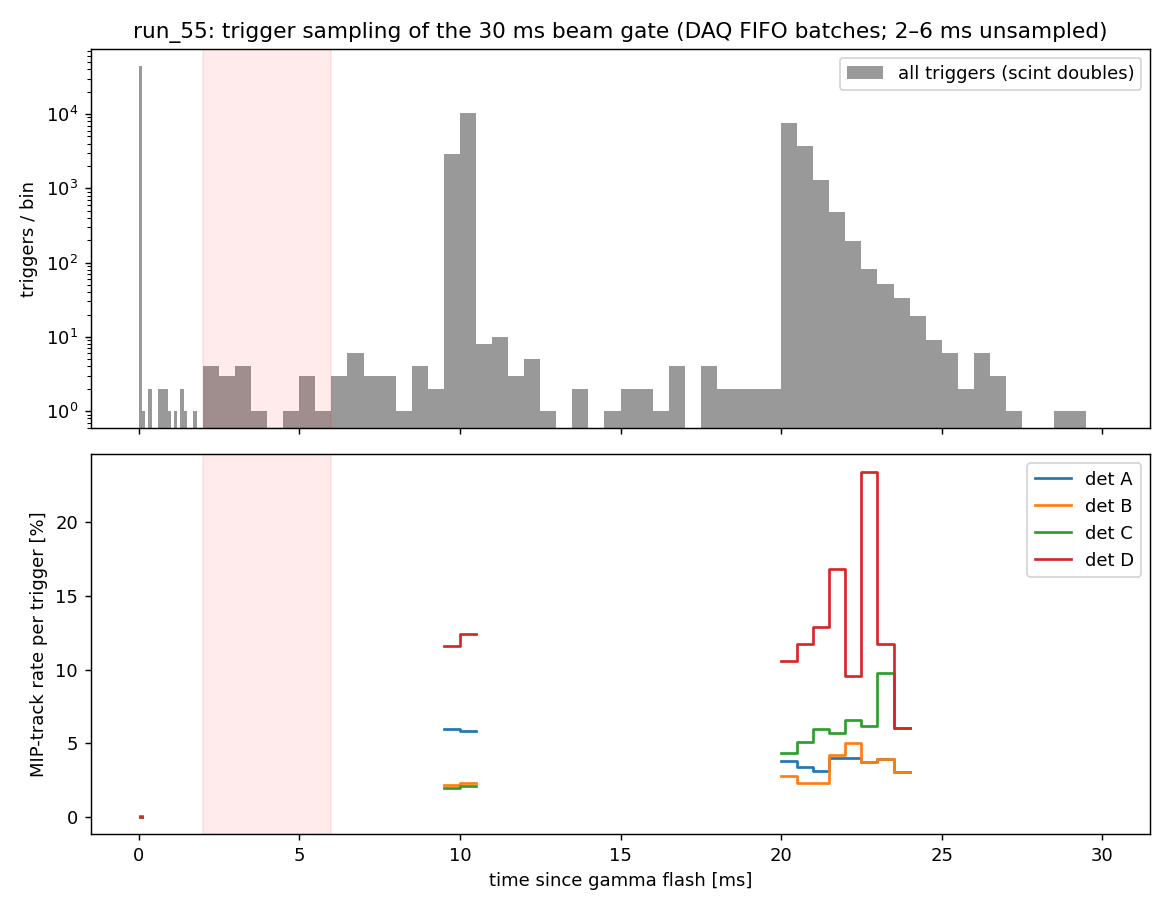
\includegraphics[width=\textwidth]{25_hv_scan/01_time_structure.png}
\column{.42\textwidth}
\begin{itemize}
\item One trigger burst per beam pulse ($\sim$3 s apart);
      \textbf{first trigger of a burst = gate open = $\gamma$ flash} ($t_0$).
      Valid for all bursts (batch structure identical whether the MM
      recorded the flash or railed empty).
\item \alert{No-ZS events are $\sim$1.6 MB $\Rightarrow$ FIFO comb}: 4--5
      events at 0--0.5 ms, dead $\sim$8 ms, batch at
      \textbf{8--12 ms} (b1), batch at \textbf{16--28 ms} (b2).
\item \alert{\textbf{2--6 ms after flash --- including the 3 ms physics
      target --- was never sampled.}}
\end{itemize}
\end{columns}
\end{frame}

\begin{frame}{The $^3$He capture flood (dominant systematic)}
\begin{columns}
\column{.52\textwidth}
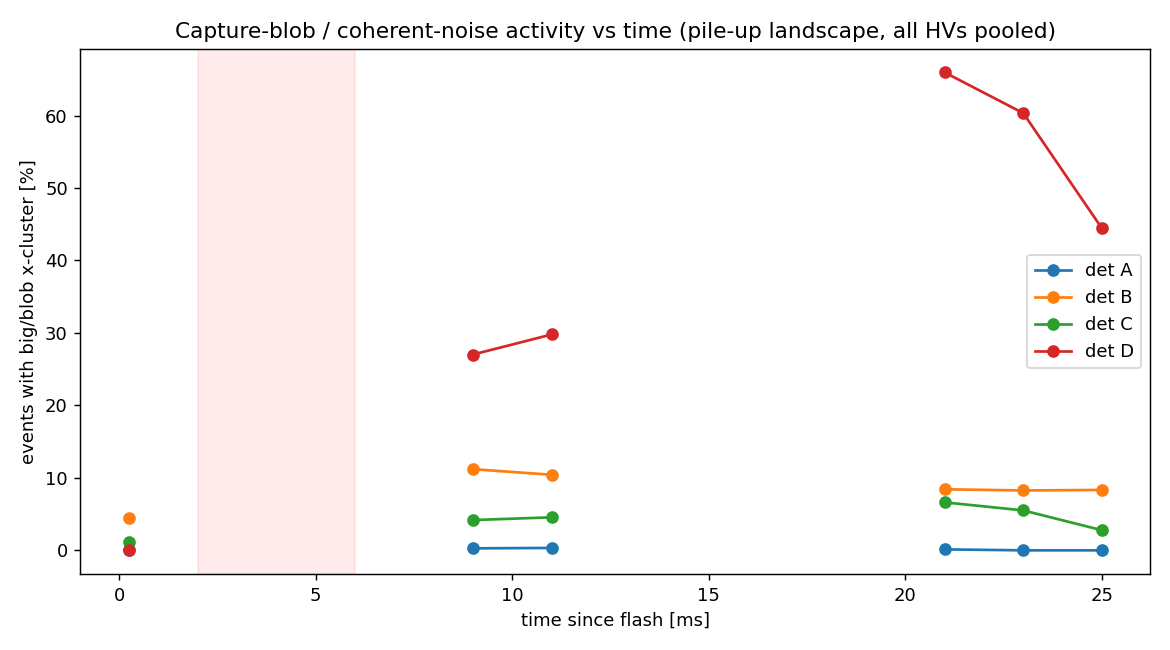
\includegraphics[width=\textwidth]{25_hv_scan/07_blob_activity.png}
\column{.46\textwidth}
\small
\begin{itemize}
\item 19 m flight path / 2200 m/s $\Rightarrow$ thermal neutrons arrive at
      \textbf{8.6 ms} --- batch b1 sits ON the thermal peak; b2 is
      sub-thermal.
\item n$+^3$He$\to$p$+$t (764 keV, heavily ionizing, mm--cm range):
      wide high-charge \textbf{blobs} in the MM windows.
\item Det D: capture-scale cluster in \textbf{$\gtrsim$90\%} of late
      windows. Arms are equidistant (pinwheel) --- D's $\sim$2$\times$
      gain is the likely reason it \emph{sees} so many more.
\item Blobs fake/mask tracks $\Rightarrow$ keep top-5 clusters/plane;
      ``MIP-like'' = 3--20 strips, $\leq$25 mm, x/y sample-coherent.
\end{itemize}
\end{columns}
\end{frame}

% ---------------------------------------------------------------- Q1
\begin{frame}{Q1a --- turn-on: dead at the flash, everywhere}
\centering
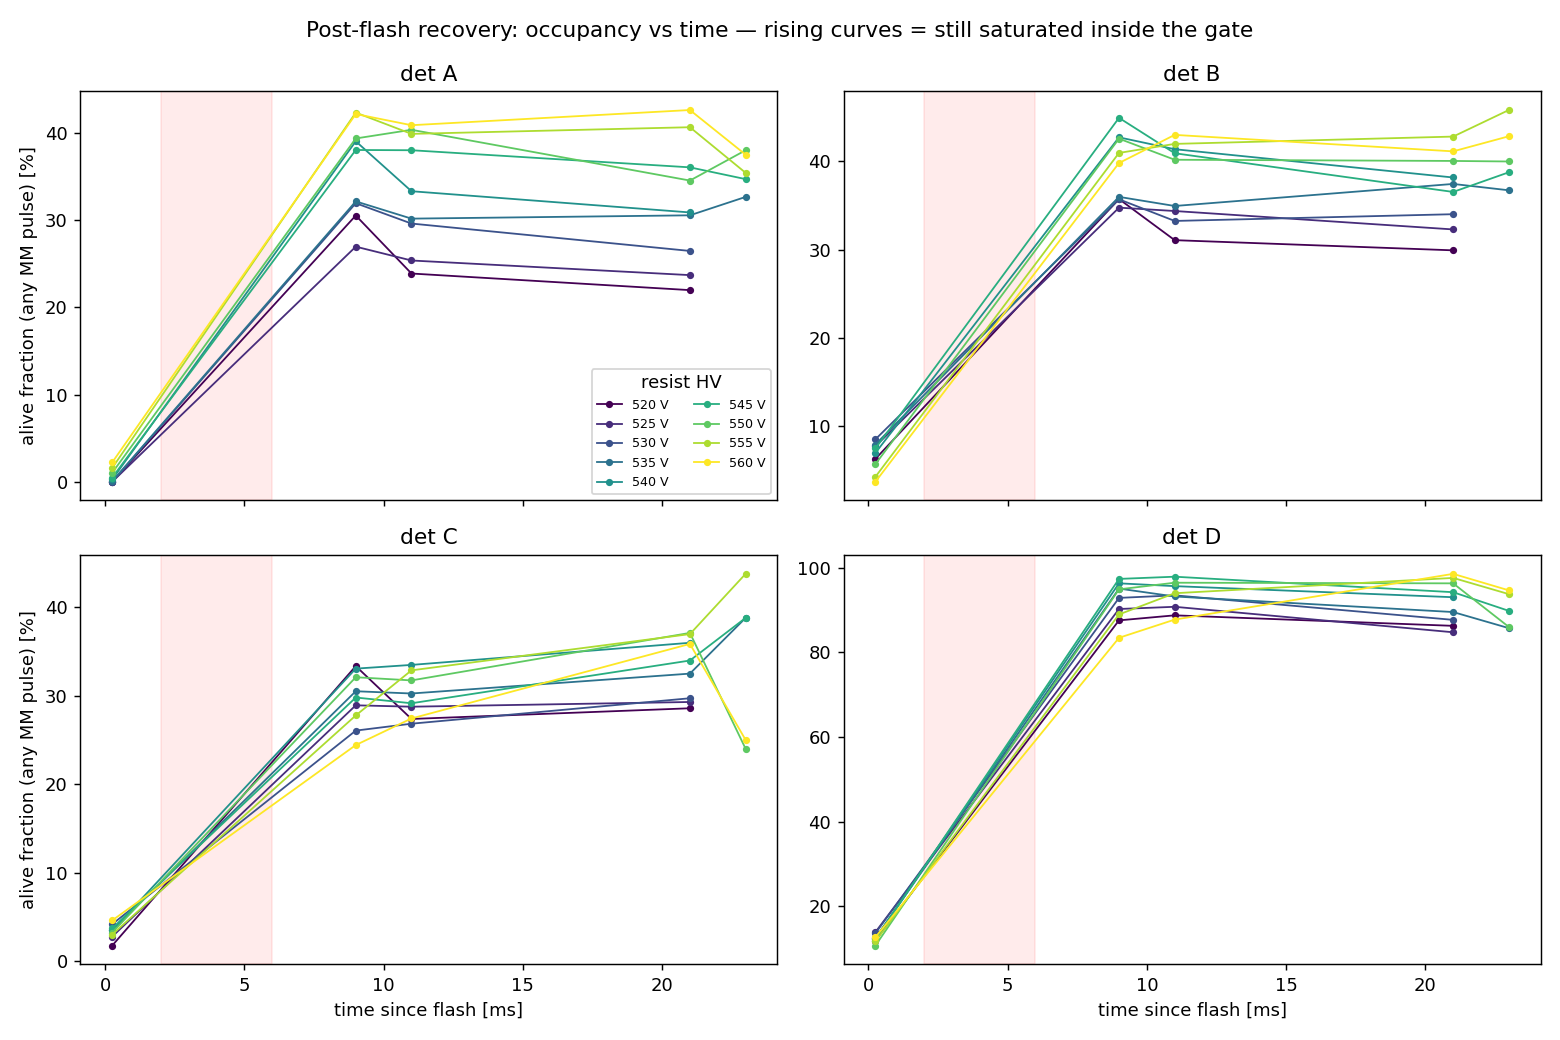
\includegraphics[width=.72\textwidth]{25_hv_scan/08_alive_recovery.png}

\vspace{1ex}
\raggedright
\textbf{0--0.5 ms: 0 tracks in 44\,686 triggers}; occupancy 0--7\%
(D $\sim$12\% = its capture flood). Scint trigger rate itself is flat across
the gate --- this is purely an MM outage.
\alert{Rising curves (C, D at 555--560 V) = still saturated at 10 ms,
recovered by $\sim$20 ms.}
\end{frame}

\begin{frame}{Q1b --- MIP-track rate vs time, per HV}
\centering
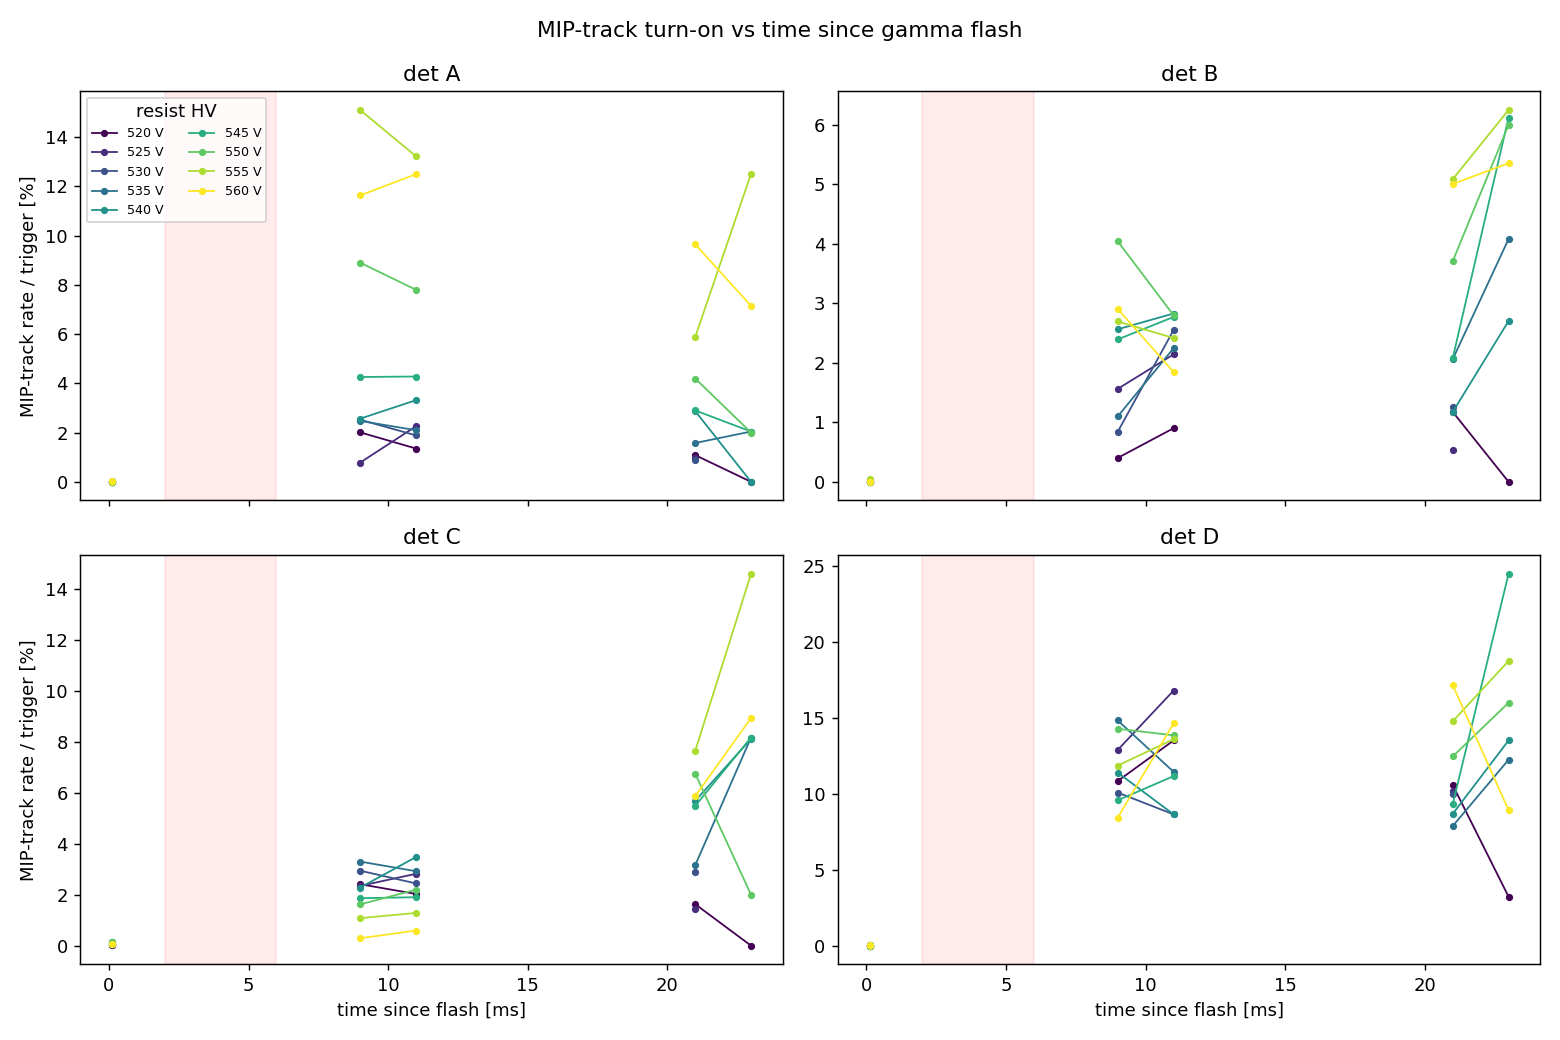
\includegraphics[width=.8\textwidth]{25_hv_scan/02_turnon_vs_time.png}
\end{frame}

\begin{frame}{Q1c --- saturation time GROWS with HV}
\begin{columns}
\column{.48\textwidth}
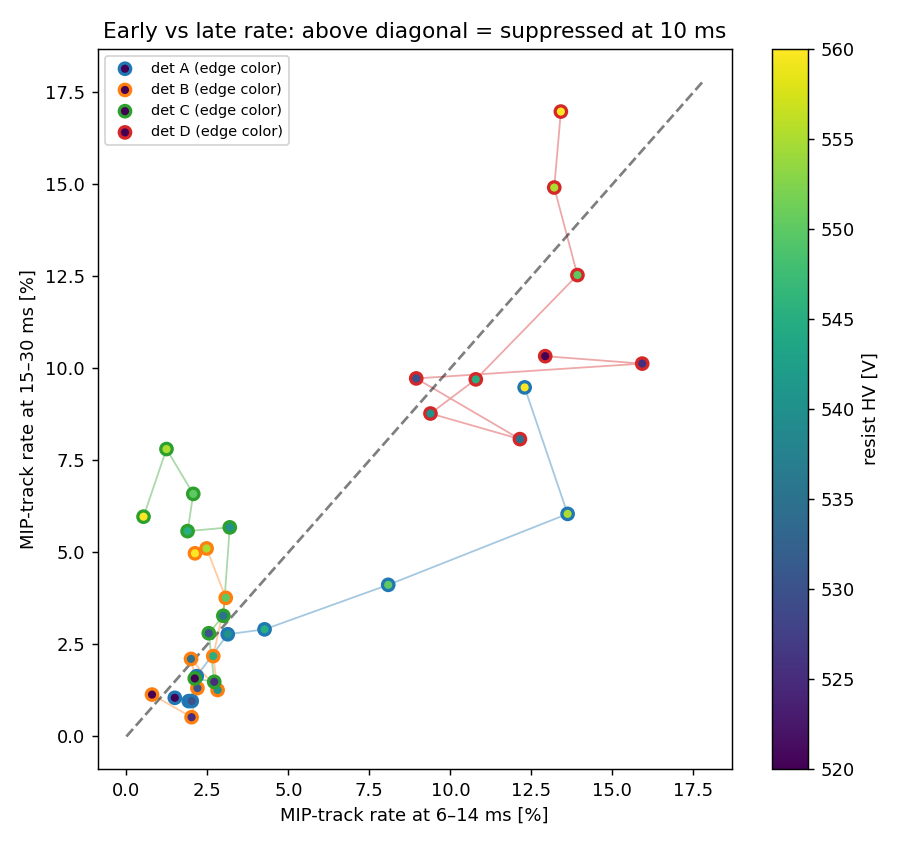
\includegraphics[width=\textwidth]{25_hv_scan/09_early_vs_late.png}
\column{.5\textwidth}
\begin{itemize}
\item $\leq$550 V: rates and occupancy flat b1$\to$b2 --- recovered before
      8 ms at every det.
\item \textbf{C at 555--560 V}: 0.5--1.2\% at 8--12 ms vs 5.9--7.8\% at
      $>$15 ms (points far \emph{above} the diagonal) --- gain still sagged
      at 10 ms.
\item \textbf{D at 560 V}: same signature, milder (occupancy
      83\%$\to$98\% through the gate).
\item \textbf{A}: points \emph{below} the diagonal --- efficiency
      \emph{declines} through the gate (13.6\%$\to$6.1\% at 555 V).
      Open; candidate: space charge in the 600 V drift under thermal load.
\item Early amplitude ``suppression'' appears as \textbf{rate loss +
      survivor bias} (only the Landau tail clears threshold), not low
      medians.
\end{itemize}
\end{columns}
\end{frame}

% ---------------------------------------------------------------- Q2
\begin{frame}{Q2a --- efficiency proxy vs resist HV (the money plot)}
\centering
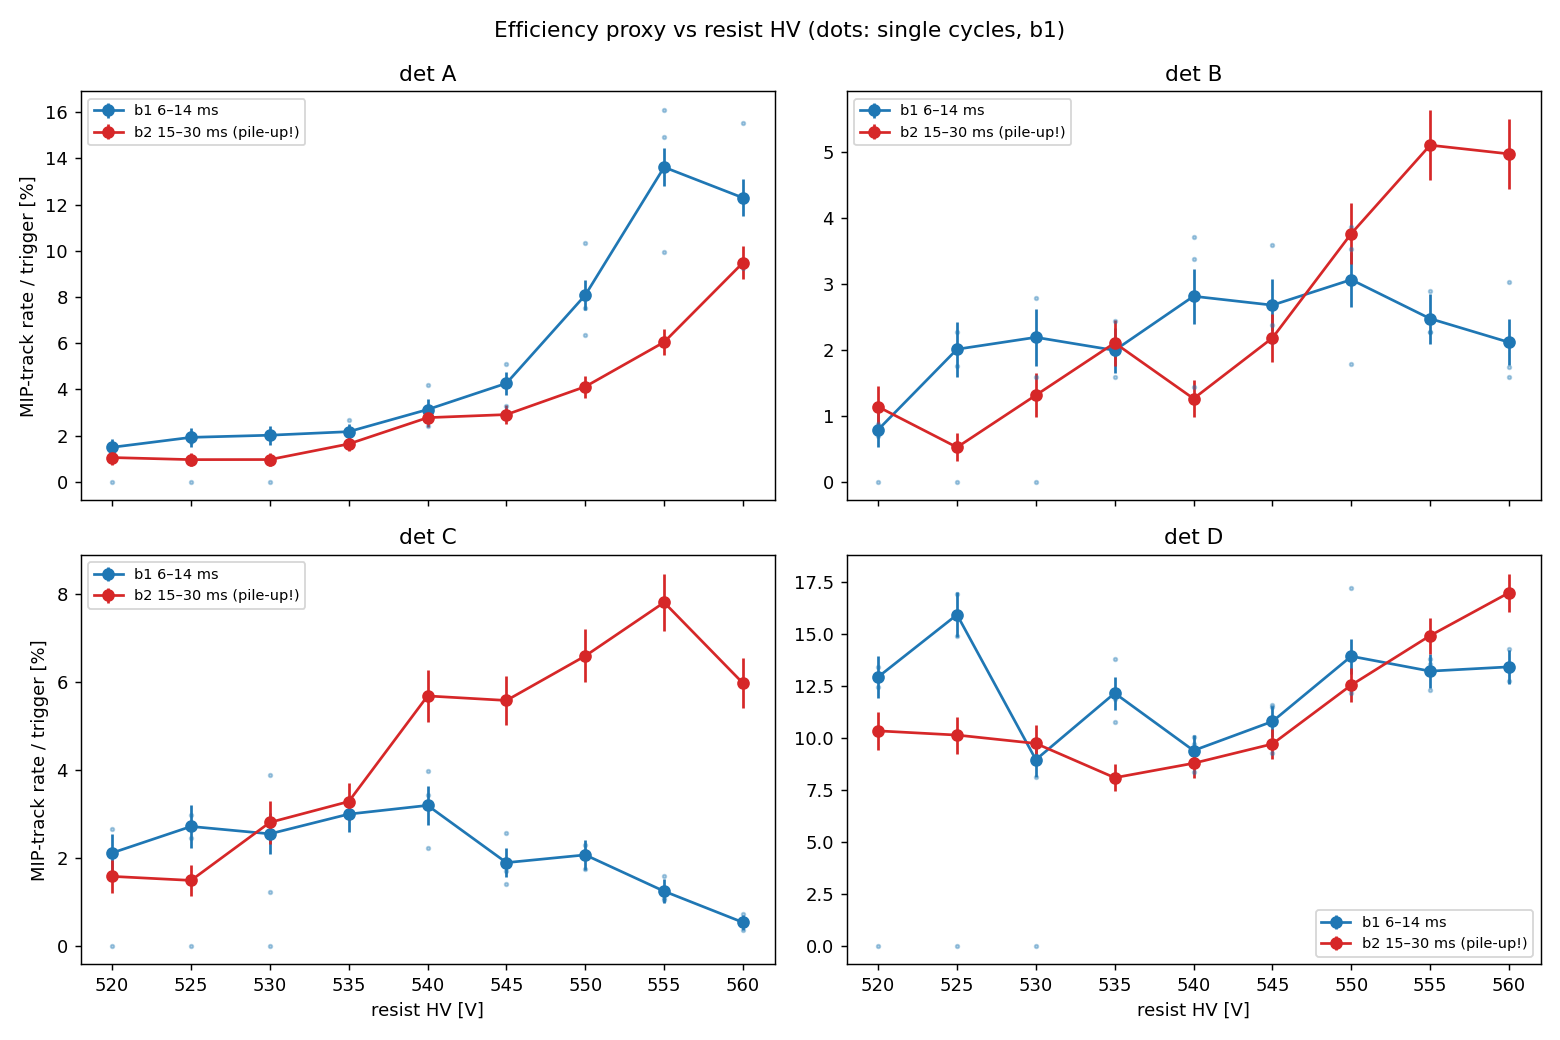
\includegraphics[width=.78\textwidth]{25_hv_scan/03_eff_vs_hv.png}
\end{frame}

\begin{frame}{Q2b --- reading the efficiency curves}
\small
\begin{columns}
\column{.5\textwidth}
MIP-track rate per trigger at 8--12 ms [\%] (geometric ceiling per arm
$\sim$50\%, doubles trigger):

\vspace{0.5ex}
\begin{tabular}{lrrrr}
\toprule
HV & A & B & C & D$^{*}$\\
\midrule
520 &  1.5 & 0.8 & 2.1 & 12.9\\
530 &  2.0 & 2.2 & 2.5 &  8.9\\
540 &  3.1 & 2.8 & 3.2 &  9.4\\
550 &  8.1 & 3.1 & 2.1 & 13.9\\
555 & \textbf{13.6} & 2.5 & 1.2 & 13.2\\
560 & 12.3 & 2.1 & 0.5 & 13.4\\
\bottomrule
\end{tabular}
\column{.48\textwidth}
\begin{itemize}
\item \textbf{A}: clean rise, \alert{no plateau by 560 V}, and NO
      saturation sag even at 560 --- simply under-biased.
\item \textbf{B}: weak response 2--3\%; late-gate rises to $\sim$5\% at
      555--560. Complicated by its wide ($\sim$200 mm) low-amp
      ringing clusters. Inconclusive.
\item \textbf{C}: true gain peak $\geq$555 V (late-gate), but
      long-saturation penalty above 550.
\item \textbf{D$^{*}$}: contaminated by capture fragments at low HV
      (13\% at 520 V is NOT MIP efficiency); plateau-ish 545--560.
\end{itemize}
\end{columns}
\end{frame}

\begin{frame}{Amplitudes: medians are threshold-biased; spectra + gain notes}
\begin{columns}
\column{.5\textwidth}
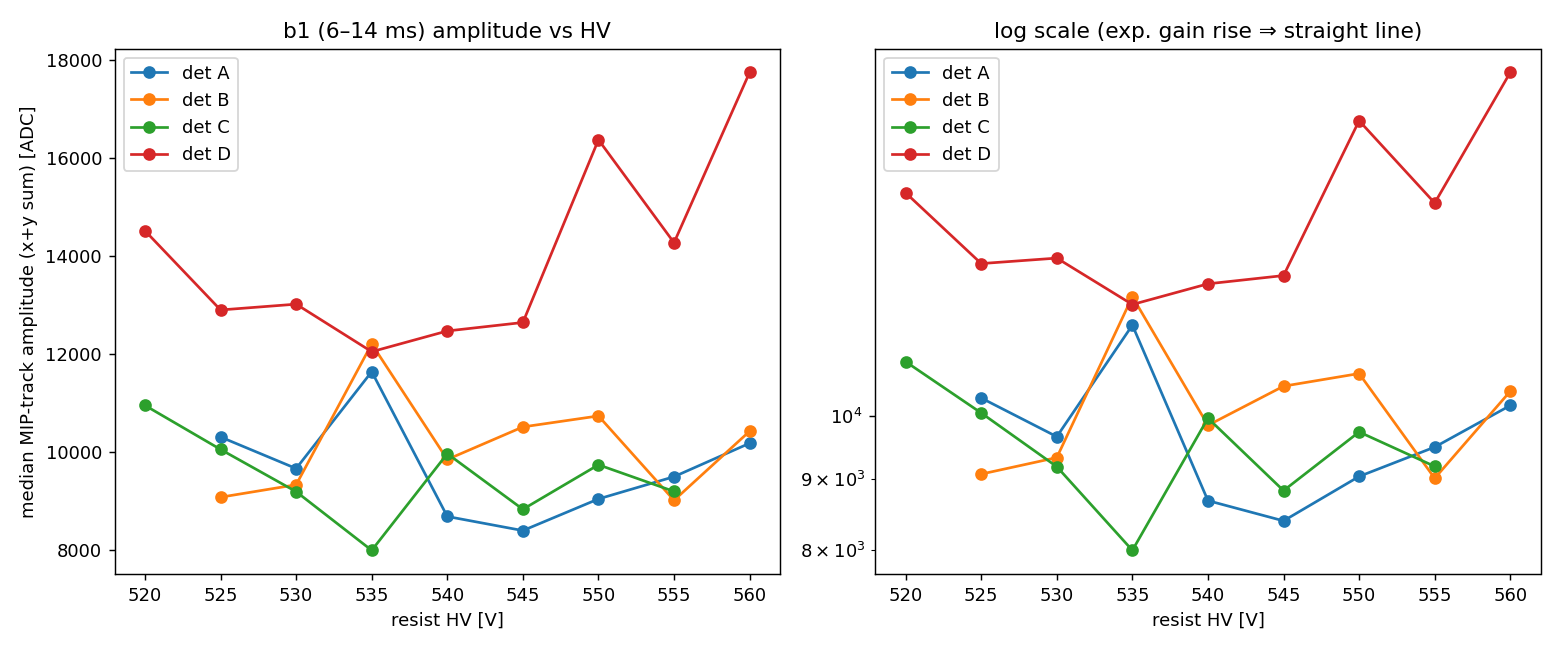
\includegraphics[width=\textwidth]{25_hv_scan/04_amp_vs_hv.png}
\column{.48\textwidth}
\begin{itemize}
\item Median MIP-track amp sits at 8--12k ADC (x$+$y) at every HV ---
      only tracks \emph{above detection} enter, so this is NOT a gain
      curve.
\item Real gain slope from D's resist current: 1.0$\to$5.4 $\mu$A over
      520$\to$560 V $\Rightarrow$ \textbf{gain doubles every
      $\sim$17 V}. (A's current is leakage-dominated: 2.7$\to$3.7 $\mu$A.)
\item Where sag exists, b1 medians are biased \emph{high}
      (ratio up to 1.3--1.4 vs b2) --- survivor bias, consistent with
      suppressed gain early.
\end{itemize}
\end{columns}
\end{frame}

\begin{frame}{Amplitude vs time and b1 spectra}
\begin{columns}
\column{.5\textwidth}
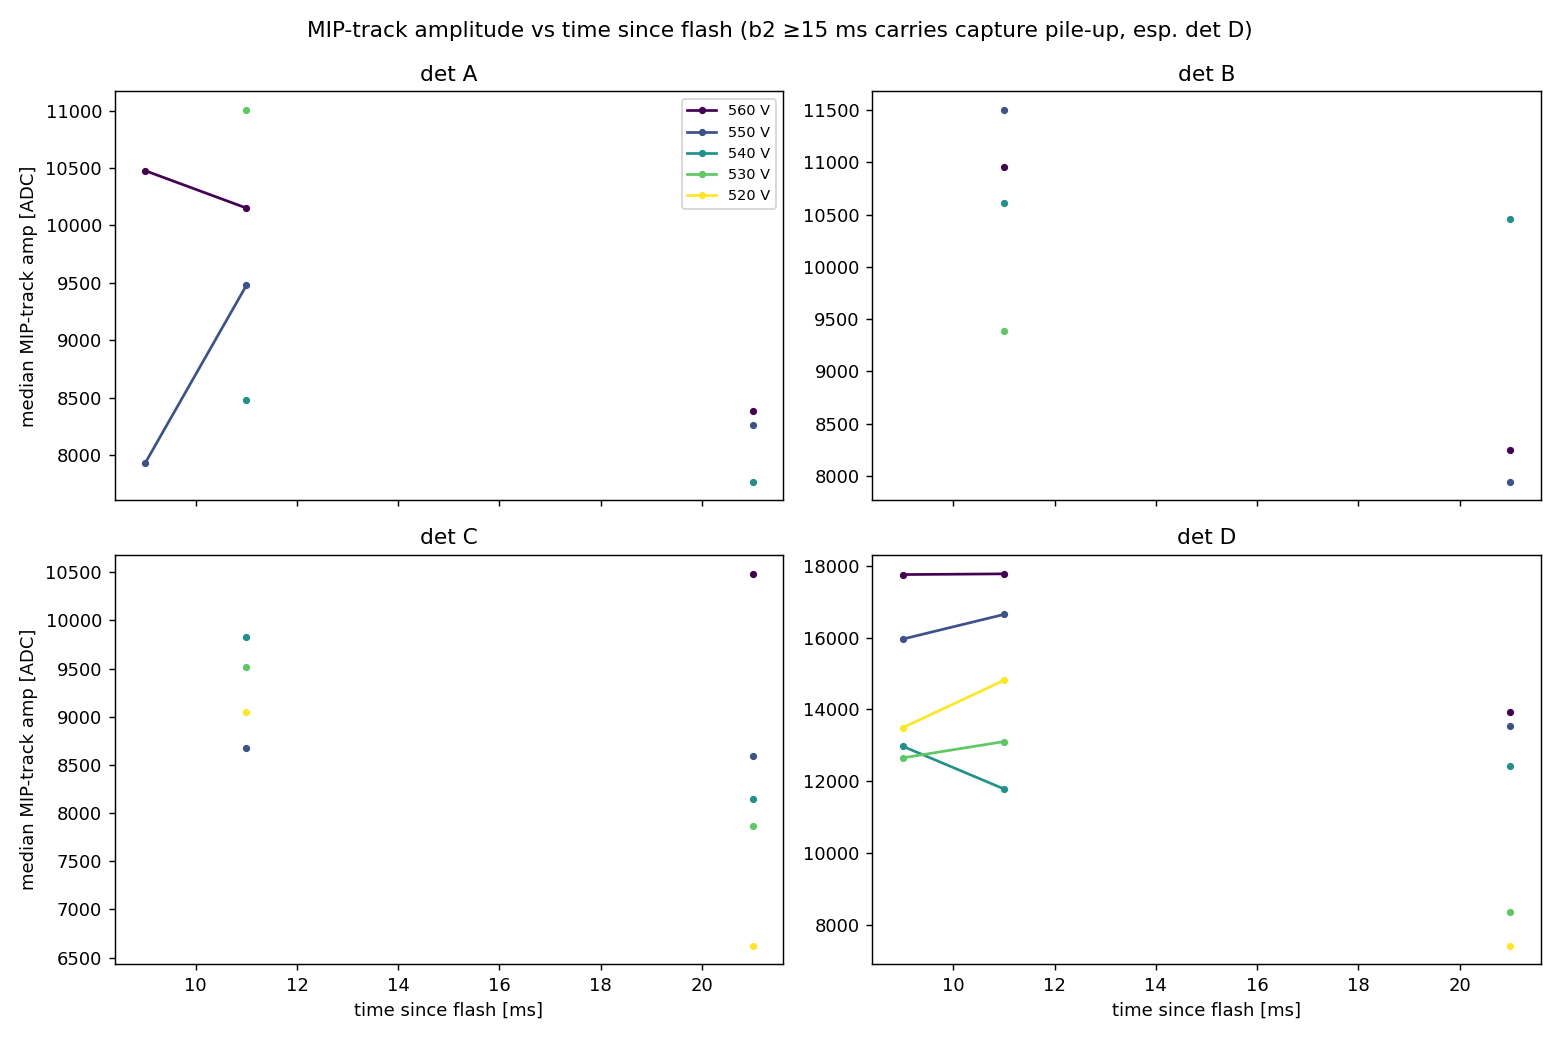
\includegraphics[width=\textwidth]{25_hv_scan/05_amp_vs_time.png}
\column{.5\textwidth}
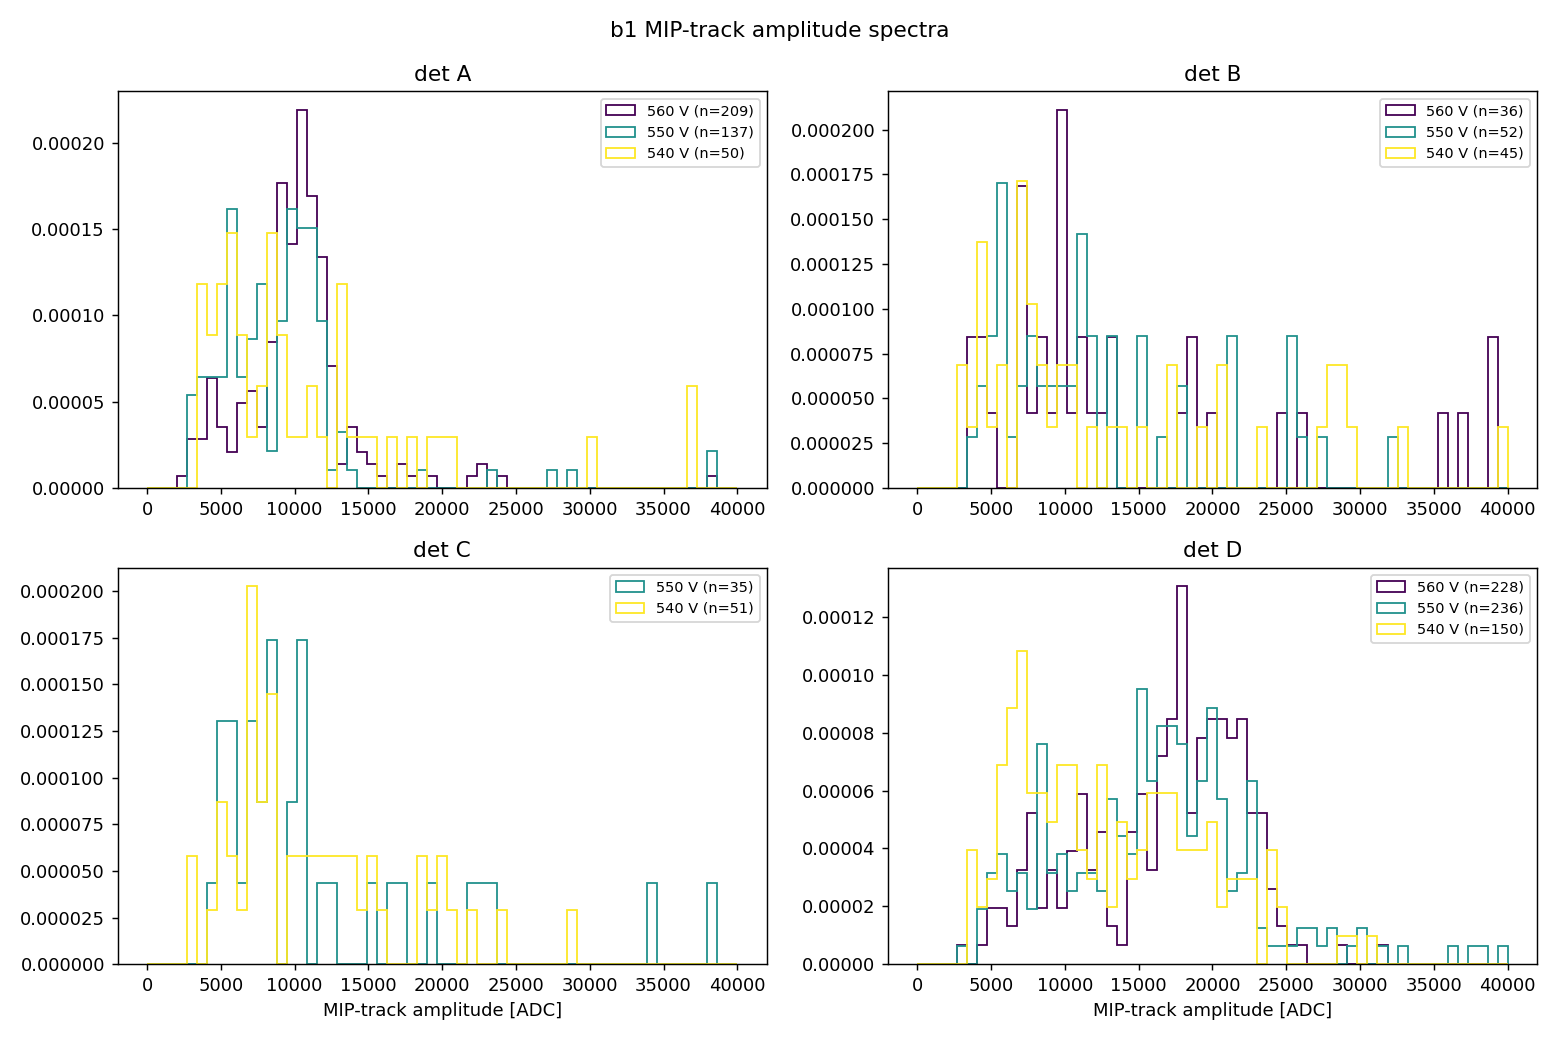
\includegraphics[width=\textwidth]{25_hv_scan/06_amp_spectra_b1.png}
\end{columns}
\end{frame}

% ---------------------------------------------------------------- clusters
\begin{frame}{Cluster multiplicity vs time and HV}
\centering
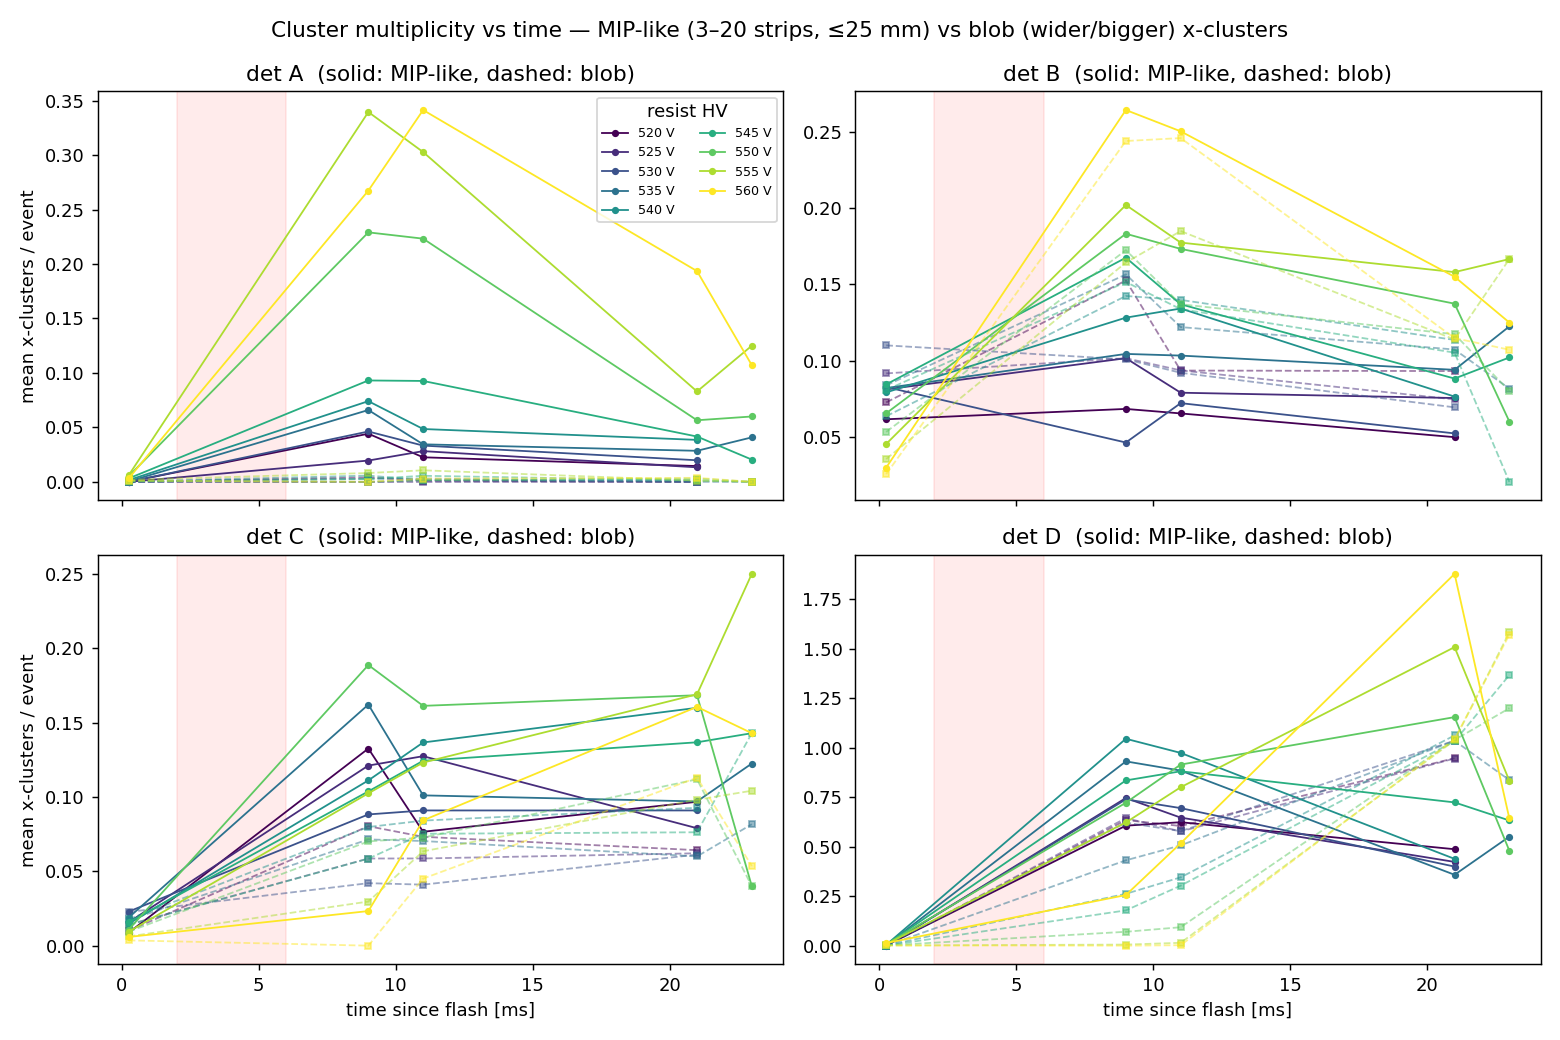
\includegraphics[width=.8\textwidth]{25_hv_scan/10_cluster_multiplicity.png}
\end{frame}

\begin{frame}{Cluster composition at 8--12 ms: four different detectors}
\centering
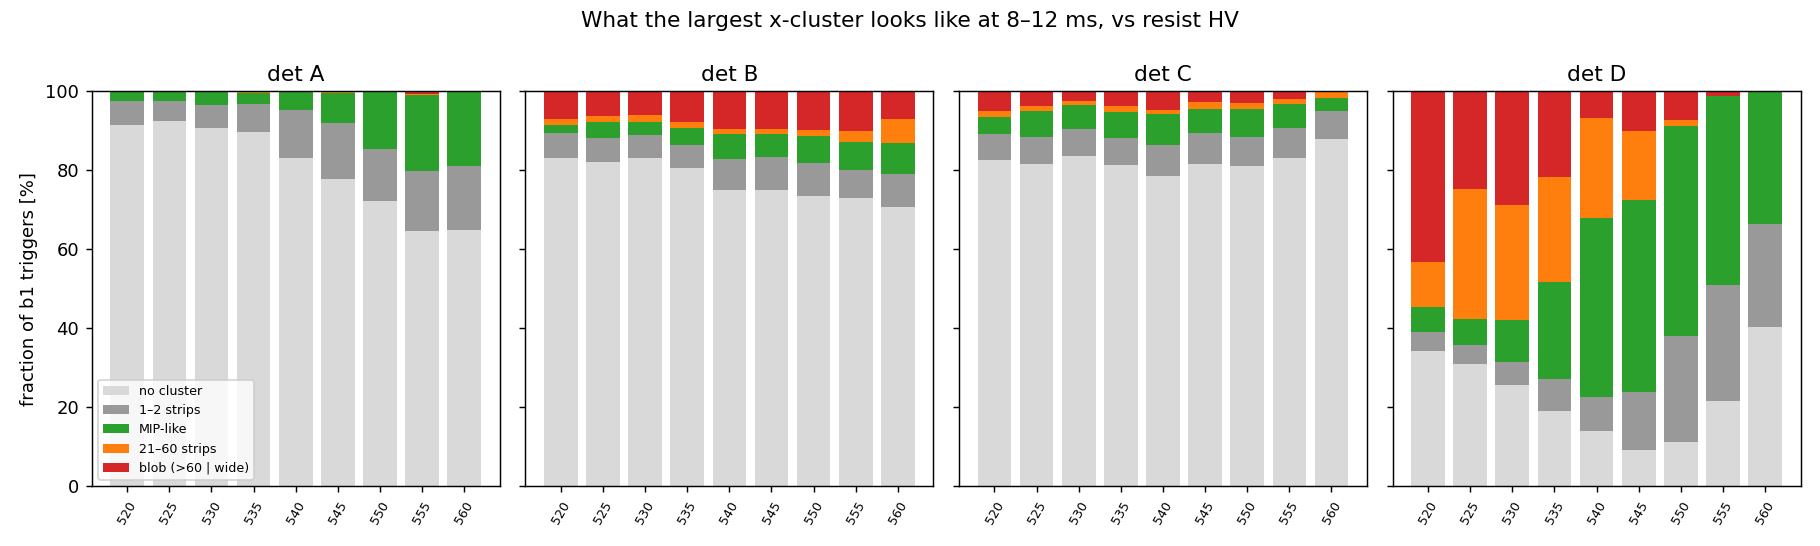
\includegraphics[width=\textwidth]{25_hv_scan/11_cluster_classes.png}

\vspace{0.5ex}
\raggedright\small
A: MIP fraction grows cleanly with HV, almost no blobs. B/C: modest MIP
fractions $+$ persistent blob/ringing background; C's dead fraction
\emph{grows} at 555--560 (sag). D: capture blobs (red/orange) at low HV
morph into MIP-class $+$ ``no cluster'' at 555--560 --- FEU saturation
fragmentation $+$ gain sag.
\end{frame}

% ---------------------------------------------------------------- summary
\begin{frame}{Recommendation (for $\geq$3 ms operation, this gas/config)}
\begin{tabular}{llp{7.2cm}}
\toprule
det & operating point & why\\
\midrule
A & \textbf{$\geq$560 V}, scan higher & rate still rising at 560; no sag
    even at 560. Drift capped at 600--700 V (sparks at 800) --- consider
    pushing drift to 700 as well\\
B & \textbf{550--555 V} (tentative) & late-gate gain still rising to 555;
    no strong sag; blocked on the ringing/wide-cluster issue\\
C & \textbf{545--550 V} & gain wants $\geq$555 but saturation
    $>$10 ms there; 545--550 = best early-gate efficiency\\
D & \textbf{540--550 V} & plateau by $\sim$545; sag at 560; full capture
    visibility everywhere\\
\bottomrule
\end{tabular}

\vspace{1.5ex}
\alert{Caveat: 3 ms itself was never sampled. At 555+ V, C/D are provably
NOT recovered at 8--12 ms --- the 3 ms goal likely requires the lower
operating points, or a saturation fix.}
\end{frame}

\begin{frame}{Open items / follow-up wanted}
\begin{itemize}
\item \textbf{Sample 1--8 ms}: rerun with zero-suppression ON (or short
      window) to shrink the $\sim$8 ms readout dead time, or step a delayed
      trigger gate through 1--8 ms. Only way to answer ``alive at 3 ms''.
      \emph{(Waiting on DAQ machine repair.)}
\item \textbf{Det A in-gate decline} (b1$\to$b2): dedicated look; space
      charge in the 600 V drift is the prime suspect --- test at drift 700 V.
\item \textbf{Det B ringing / wide clusters}: waveform-level diagnosis
      (needs \texttt{raw\_daq\_data} or \texttt{hits\_root}, still on EOS).
\item Higher-HV point for A (565--575 V) to find its plateau.
\item Absolute per-arm efficiency: tag-and-probe across arms from the
      doubles trigger (16-pattern likelihood; machinery in
      \texttt{ntof\_tracking/}).
\end{itemize}
\end{frame}

\end{document}
